\documentclass[14pt, a4paper]{extarticle}

\usepackage{cmap}
\usepackage{mathtext}
\usepackage[T2A]{fontenc}
\usepackage[utf8]{inputenc}
\usepackage[english, russian]{babel}
\usepackage{indentfirst}
\frenchspacing

\usepackage{amsmath, amssymb, amsfonts, amsthm, mathtools}
\usepackage{icomma}

\usepackage{centernot}
\usepackage{stmaryrd}

\renewcommand{\epsilon}{\ensuremath{\varepsilon}}
\renewcommand{\phi}{\ensuremath{\varphi}}
\renewcommand{\kappa}{\ensuremath{\varkappa}}
\renewcommand{\le}{\ensuremath{\leqslant}}
\renewcommand{\leq}{\ensuremath{\leqslant}}
\renewcommand{\ge}{\ensuremath{\geqslant}}
\renewcommand{\geq}{\ensuremath{\geqslant}}
\renewcommand{\emptyset}{\ensuremath{\varnothing}}

\usepackage{graphicx}
\usepackage{wrapfig}

\usepackage{array, tabularx, tabulary, booktabs}
\usepackage{longtable}
\usepackage{multirow}

\theoremstyle{definition}
\newtheorem{theorem}{Теорема}[section]
\newtheorem{lemma}{Лемма}[section]
\newtheorem{proposition}{Утверждение}[section]
\newtheorem*{exercise}{Упражнение}
\newtheorem{problem}{}

\theoremstyle{definition}
\newtheorem{definition}{Определение}[section]
\newtheorem*{corollary}{Следствие}
\newtheorem*{note}{Замечание}
\newtheorem*{reminder}{Напоминание}
\newtheorem*{example}{Пример}

\theoremstyle{remark}
\newtheorem*{solution}{Решение}

\usepackage{geometry}
\usepackage{setspace}
% \usepackage{enumitem}
\usepackage[inline]{enumitem}
\setlist{leftmargin=25pt}

\geometry{top=20mm}
\geometry{bottom=15mm}
\geometry{left=15mm}
\geometry{right=15mm}

\setlength\parindent{15pt}
\linespread{1.3}

\usepackage{multicol}
\usepackage{soulutf8}

\usepackage{microtype}

\usepackage{tocloft}

\makeatletter
\def\eqref{\@ifstar\@eqref\@@eqref}
\def\@eqref#1{\textup{\tagform@{\ref*{#1}}}}
\def\@@eqref#1{\textup{\tagform@{\ref{#1}}}}
\makeatother
\numberwithin{equation}{section}
\mathtoolsset{showonlyrefs=false}

\usepackage{hyperref}
\usepackage[usenames,dvipsnames,svgnames,table,rgb]{xcolor}
\hypersetup{
    unicode=true,
    colorlinks=true,
    linkcolor=black!15!blue,
    citecolor=green,
    filecolor=magenta,
    urlcolor=NavyBlue,
}

\usepackage{tikz}
\usepackage{tikz-cd}
\usepackage{tkz-euclide}
\usepackage{stackengine}
\usetikzlibrary{angles, babel, quotes}

% \usepackage{paratype}
% \usepackage{euler}

\newcommand{\N}{\ensuremath{\mathbb{N}}}
\newcommand{\Z}{\ensuremath{\mathbb{Z}}}
\newcommand{\Q}{\ensuremath{\mathbb{Q}}}
\newcommand{\R}{\ensuremath{\mathbb{R}}}

\usepackage[normalem]{ulem}
\usepackage{fancyhdr}

\usepackage{graphicx}
\usepackage{wrapfig}
\usepackage{tikz}
\usepackage{listings}

\pagestyle{fancy}
\fancyhf{}
\fancyhead[R]{\href{https://vk.com/pr0st0_sasha}{Автор}}
\fancyhead[L]{\href{https://t.me/argumentofperiapsis}{\TeXподдержка}}
\chead{\textbf{Приемка ФПМИ 2023}}

% ---------

\DeclareRobustCommand{\divby}{%
  \mathrel{\text{\vbox{\baselineskip.65ex\lineskiplimit0pt\hbox{.}\hbox{.}\hbox{.}}}}%
}

\begin{document}

\subsection*{Задачи по информатике}

\begin{problem}
    Дан отсортированный массив целых чисел, вывести 
    отсортированный массив их квадратов.
\end{problem}

\begin{problem}
    Построй очередь на двух стеках.
\end{problem}

\begin{problem}
    Двое играют в игру: нужно по очереди класть на прямоугольный
    стол пятирублевые моненты. Если один не может положить 
    монету, то победа засчитывается второму.

    Может ли какой-то из игроков гарантированно победить? Если может,
    то предложи стратегию.
\end{problem}

\begin{problem}
    \textit{Студент1} и \textit{Студент2} прогневали правителя
    здешних земель --- А.Д. Поселочного. Им грозит смертная казнь.
    Однако властитель оказался милосердный. Он предложил
    им следующее: их ведут в темницу и разводят по одиночным камерам,
    там они бросают монетку, а далее каждый должен сказать,
    что выпало у товарища. Если хотя бы один угадывает, их отпускают, 
    иначе ...

    У товарищей есть пару минут, пока их ведут в камеры, чтобы 
    обсудить стратегию. Итак вопрос: смогут ли они гарантированно выйти
    живыми и невредимыми?
\end{problem}

\begin{problem}
    1,5 землекопа из \textit{страны невыученных уроков} копали-копали яму
    и вдруг наткнулись на какой-то корешок. Пригляделись внимательно,
    куда он ведет, и увидели огромное бинарное дерево. И, по всем канонам
    этой чудесной страны, дерево оказалось не простым, а золотым 
    (каждая его нода
    содержала \textit{целое} количество золота). Они решили пройтись 
    по дереву и по максимуму собрать золота. Они могут
    стартовать в любой ноде, а дальше двигаться вперед или назад. 
    Однако возвращаться в уже посещенную ими ноду категорически 
    запрещено. Как им лучше поступить?

    \textit{Предложить решение за линию.}

    // Вставить картику с деревом
\end{problem}

\begin{problem}
    Принц-Полукровка оставил в своем учебнике по зельеварению 
    огромное число подсказок и заметок. Одна из заметок содержала 
    "Закон несохранения массы". Далее идет ее текст.

    \textit{Посмотрим на веса каждого из ингредиентов в рецепте и 
    каждому из них сопоставим столбик единичной ширины и высоты, 
    равной числу граммов соответствующего ингредиента. 
    Выровняем их снизу по одной линии и получим "гистограмму 
    ингредиентов". Тогда масса полученного зелья будет равняться 
    площади самого большого прямоугольника в гистограмме, одна 
    из сторон которого лежит на общей нижней линии.}

    Найди площадь самого большого прямоугольника в гистограмме. 
    Помни, что этот прямоугольник должен быть на общей базовой линии.

    // Вставить пример гистограммы
\end{problem}

\begin{problem}
    Есть односвязный список, состоящий из различных значений. 
    Возможно в нем есть цикл. Опиши алгоритм, который находит
    начало этого цикла, а если цикла нет --- выводит \textit{-1}.

    \begin{tikzpicture}[->,>=stealth,shorten >=1pt,auto,
        node distance=2.5cm, thick,
        main node/.style={circle,draw,font=\sffamily\Large\bfseries}]

    % Nodes
    \node[main node] (1) {1};
    \node[main node] (2) [right of=1] {4};
    \node[main node] (3) [right of=2] {2};
    \node[main node] (4) [right of=0.5cm of 3, above of=3] {3};
    \node[main node] (5) [right of=4, below of=4] {5};
    \node[main node] (6) [below of=4, below of=4] {6};

    % Edges
    \path[every node/.style={font=\sffamily\small}]
    (1) edge (2)
    (2) edge (3)
    (3) edge (4)
    (4) edge (5)
    (5) edge (6)
    (6) edge (3);

    \end{tikzpicture}
\end{problem}

\begin{problem}
    Вагоны новой кольцевой железной дороги было предложено расписать 
    $N$ дизайнерам. Каждый дизайнер выбирал для своей раскраски полосу 
    длиной $L_i$, начинающуюся от начала вагона и гарантированно 
    помещающуюся на вагоне. Тем самым какие-то работы были полностью 
    закрашены, а какие-то всё же были видны хотя бы частично.

    Тебе дана последовательность перекраски. После завершения работы 
    каждого дизайнера выведи одно число — количество различных работ, 
    элементы которых видны на момент завершения.

    \textit{Предложить решение за линию.}
\end{problem}

\begin{problem}
    \textbf{Король и вино.}

    Представь, ты --- король, и у тебя завтра день рождения. По такому случаю ты устраиваешь
    вечеринку! Но какая же вечеринка может обойтись без открытия винного погреба?)
    И вот ты спускаешься в свой погреб и обнаруживаешь в нем ... записку, в которой говорится,
    что одна из 1000 бутылок вина отравлена. Яд этот очень опасный и всего одна его капля
    способна убить человека всего за 15-20 часов. И всё бы было не так плохо, да вот до праздника
    остается всего один день! 
    
    Подвергать риску себя и своих гостей ты не можешь, зато у тебя 
    в темнице множество узников, которые ждут своей казни. И ты решаешь дать им вина,
    чтобы вычислить отравленную бутылку. Человек ты сердобольный, поэтому тебе хочется подвергнуть
    риску как можно меньшее количество заключённых. Вопрос: какое минимальное количество 
    заключённых должно попробовать вино из бутылок, чтобы точно найти отравленную в течение 24 часов?
\end{problem}

\begin{problem}
    \textbf{Infinity Train}

    Представь замкнутую по окружности железную дорогу. 
    По ней едет поезд, последний вагон которого скреплён с первым так, 
    что внутри можно свободно перемещаться между вагонами. 
    Ты оказался в каком-то случайном вагоне и твоя задача — \textit{посчитать 
    их общее количество}. В каждом вагоне можно включать или выключать 
    свет, но начальное положение переключателей случайное и заранее неизвестно.

    Все вагоны внутри выглядят одинаково, окна закрыты так, что невозможно 
    посмотреть наружу, движение поезда равномерное. Помечать вагоны как-либо, 
    кроме включения или выключения света, нельзя. 
    Количество вагонов конечно (не верьте заголовку).

    \textit{Придумать решение за линию.}
\end{problem}

% -------
\subsection*{Задачи по математике}
\setcounter{problem}{0}

\begin{problem}
    Можно ли торт 3 разрезами поделить на 8 частей.
\end{problem}

\begin{problem}
    В кубической комнате со стороной 2 летают 9 мух. 
    Докажи, что найдется хотя бы одна пара мух, 
    находящихся на расстоянии не большем $\sqrt{3}$.
\end{problem}

\begin{problem}
    У шахматной доски отрезали два противолежащих уголка.
    Можно ли теперь покрыть ее доминошками (по структуре они
    наполовину черные, наполовину белые)?
\end{problem}

\begin{problem}
    Решить $3\sqrt{4x - 5y + 7} +
    5|3x - 4y + 6| \leqslant 4$, где $x, y \in \Z$.
    В ответе указать $max(x+y)$.
\end{problem}

\begin{problem}
    \textbf{Читать голосом Александра Пушного.}

    В эфире самая смешивательная среди взбалтывательных и самая
    взбалтывательная среди смешивательных рубрик программы <<Галилео>>, 
    которая называется ЭЭЭЭЭЭКСПЕРИМЕНТЫ.
    
    Друзья, смотрите, мы берем две совершенно одинаковые кружки.
    В одной из них молоко, в другой --- кофе (в одинаковых количествах). 
    Переливаем ложку молока в кофе, перемешаем, 
    а затем обратно переливаем ложку получившейся смеси в стакан с молоком. 
    Итак, наши внимательные зрители, чего же у нас оказалось больше:
    молока в кофе или кофе в молоке?

    \textit{Подсказка}. Можешь для начала решить следующую задачу:

    На главную туристическую площадь приехали два туристических 
    автобуса. Все места в каждом из автобусов были заняты. 
    В первом автобусе находилось 20 польских 
    туристов, во втором --- 20 чешских. Во время экскурсии 
    начался ливень, и туристы бросились в автобусы, не разбирая, где чей. 
    Кого больше: чешских туристов в польском автобусе или польских 
    туристов в чешском?
\end{problem}

\begin{problem}
    Существует ли такой $x$, что $tg(x) + \sqrt{3}$ и 
    $ctg(x) + \sqrt{3}$ целые числа?
\end{problem}

\begin{problem}
    //Жду Федю с картинкой про геому 7 класс
\end{problem}

\begin{problem}
    Решить $2x \cdot 2^x + 3x \cdot 3^x + 1 \geqslant 
    \sqrt{4^x + 9^x +1} \cdot \sqrt{13x^2 + 1}.$
\end{problem}

\begin{problem}
    //Жду Федю с картинкой про геому 4 решения
\end{problem}

\begin{problem}
    \textbf{Ральный кейс.}

    Открывает первокурсник задавальник \sout{, а он ему как раз}
    и видит такую задачу: <<Почему $\sqrt{2}$ иррационально?>>
\end{problem}

\begin{problem}
    \begin{multicols}{2}
        Из 9 аксиом поля действительных чисел вывести следующее:
        \renewcommand{\labelenumi}{\alph{enumi})}
        \begin{enumerate}
        \item $\forall a \in \R \ \exists ! \; (-a)\in \R : a + (-a) = 0;$
        
        \item $\forall a \in \R : \ a \cdot 0 = 0;$
        
        \item $\forall a \in \R : \ (-1) \cdot a = -a.$
        \end{enumerate}

        \columnbreak

        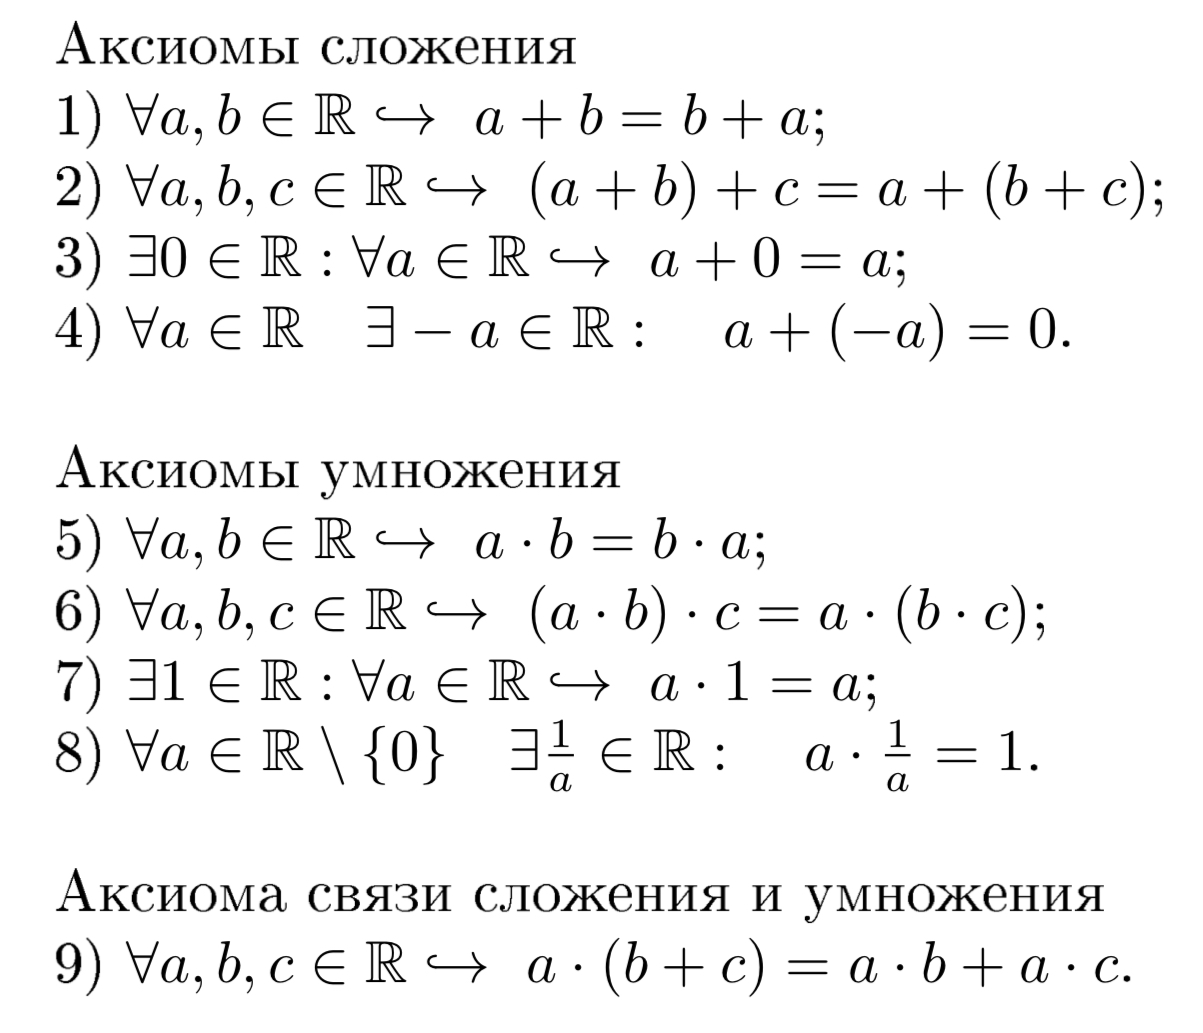
\includegraphics[width=0.46\textwidth]{ax.jpeg}
      \end{multicols}
\end{problem}

\begin{problem}
    Доказать, что $\displaystyle\lim_{n\to\infty}{\sqrt[n]{n}} = 1.$
\end{problem}

\begin{problem}
    Доказать, что $D(x) = \displaystyle\lim_{m\to\infty}{\lim_{n\to\infty}
    {\cos^{2n}(\pi \cdot m! \cdot x)}}$, где $D(x)$ - функция Дирихле.
\end{problem}

\begin{problem}
    \textbf{Бонус к первой задаче.}

    Докажите, что в $\R^2$ это невозможно.

    Здесь торт --- связное выпуклое множество в $\R^2$ 
    с топологией, порождённой евклидовой метрикой.
\end{problem}

\newpage
\section*{Решения}
\subsection*{Информатика}
\setcounter{problem}{0}

\begin{problem}
    Идейно: самые большие по модулю числа на концах.

    \textit{leftIndex = 0, rightIndex = n - 1;}

    Дальше сравниваем элементы и записываем в новый массив с конца.
\end{problem}

\begin{problem}
    stackIn, stackOut.
\end{problem}

\begin{problem}
    Идея симметрии. Первый кладет монету на центр стола, второй кладет
    куда-то, а задача первого --- симметрично отражать ходы соперника.
\end{problem}

\begin{problem}
    \textit{Подсказка.} От чего можно отталкиваться, если не знаешь, 
    что выпало у соседа?

    \textbf{Решение:} Один говорит, что выпало у него, второй --- 
    отрицание своего результата.
\end{problem}

\begin{problem}
    Через DFS посчитать максимальные пути.
    \begin{footnotesize}
        \begin{lstlisting}[language=Java]
            class Solution {
                int answer = 0;
                int maxPathSum(TreeNode root) {
                    helper (root);
                    return answer;
                }

                int helper (TreeNode node) {
                    if (node == null) {
                        return 0;
                    }
                
                    int maxLeftPath = Math.max(helper(node.left), 0);
                    int maxRightPath = Math.max(helper(node.right), 0);
                    answer = Math.max(answer, maxLeftPath + maxRightPath + node.val);
                    return Math.max(maxLeftPath, maxRightPath) + node.val;
                }
            }
        \end{lstlisting}
    \end{footnotesize}
\end{problem}

\begin{problem}
    \href{https://youtu.be/zx5Sw9130L0}{Разбор.}

    Первый проход имеет 3 базовых случая:
    \renewcommand{\labelenumi}{\alph{enumi})}
    \begin{enumerate}
        \item Слудующий столбец меньше предыдещего,
        тогда максимальная площадь --- высота первого столбца.
        \item Слудующий столбец равна предыдещего, тогда
        максимальная площадь --- удвоенная высота столбца.
        \item Слудующий столбец больше предыдещего, тогда
        максимальная площадь --- высота первого столбца, но
        продленного дальше.
    \end{enumerate}

    Тогда сделаем так: заведем два стека, в одном будут лежать индексы
    столбцов, а во втором их высоты. Будем идти по гистограмме, если 
    введенный столбец $\geqslant$ предыдущего, то записываем его в стек,
    обновляем стек индексов. Если же меньше, то попаем из стеков столбцы,
    при этом считая возможную максимальную площадь, пока не дойдем до 
    случая $\geqslant$. Индекс у последнего введенного столбца можно 
    оставить как у последнего попнутого, тк туда мы очевидно можем 
    продлиться. А после цикла еще раз пробегаемся по непопнутым значениям
    и считаем возможные макс площади для них (они все образуют строго
    возрастающую последовательность).\\

    \begin{footnotesize}
        \begin{lstlisting}[language=Java]
            public class Task {
                public static void main(String[] args) throws IOException {
                    BufferedReader bi = new BufferedReader(
                        new InputStreamReader(System.in));
                    PrintWriter pw = new PrintWriter(System.out);
                    StringTokenizer st = new StringTokenizer(bi.readLine());
                    Stack<Long> indexes = new Stack<>();
                    Stack<Long> heights = new Stack<>();
                    long maxArea = 0;
                    int N = Integer.parseInt(st.nextToken());

                    for (int i = 1; i <= N; i++) {
                        long num = Long.parseLong(st.nextToken());
                        long prevInd = i;
                        while (!heights.isEmpty() && heights.peek() > num) {
                            prevInd = indexes.peek();
                            long area = heights.pop() * (i - indexes.pop());
                            maxArea = Math.max(maxArea, area);
                        }
                        indexes.add(prevInd);
                        heights.add(num);
                    }

                    while (!indexes.isEmpty()) {
                        long area = heights.pop() * (N - indexes.pop() + 1);
                        maxArea = Math.max(maxArea, area);
                    }

                    pw.printf("%d", maxArea);
                    pw.close();
                }
            }
        \end{lstlisting}
    \end{footnotesize}
\end{problem}

\begin{problem}
    Плавно подводим к мысле об использовании двух указателей.

    Подзадача: найти середину связного списка.

    Метод Эзопа: заводим указатель-черепашку, указатель-кролика.
    У первого скорость $v$, у второго $2v$. Тогда при пробеге через
    весь список черепашка будет на середине.

    В этой задаче сначала запускаем их, если цикла нет --- ответ.
    Если есть, то рано или поздно они встретятся где-то в цикле.
    Если к этому моменту черепашка сделала $i$ шагов, а кролик $2i$,
    то их позиции совпадают с точностью до целова количества кругов
    цикла: $2i = i + k \lambda \Rightarrow i = k \lambda$.

    Далее перемещаем один указатель в начало и уравниваем скорости.
    Утверждается, что если их снова запустить, то встретятся они
    в начале цикла. Это так, ибо:
    \begin{enumerate}
        \item до начала цикла указатель из начала пройдет $j$ шагов. 
        \item черепашка прошла целое количество
        циклов $k \lambda$, и тк она стартует из начала списка, то до конца
        цикла она не проходит аккурат $j$ шагов.
    \end{enumerate}
    \textbf{Ч.Т.Д.}
\end{problem}

\begin{problem}
    Берем стек. 

    Цикл по дизайнерам:
    \begin{itemize}[]
        \item Для очередного значения $L$ снимаем с вершины элементы, пока они $\leqslant L$;
        \item Вставляем $L$;
        \item Выводим кол-во элементов стека;
    \end{itemize}
\end{problem}

\begin{problem}
    Подводим к идее пронумеровать все бутылки двоичным кодом, а дальше
    сделать таблицу, где в столбцах указываются номера бутылок, 
    соответственно по столбцу пишем их номер в двоичной СС, в строках
    будут просто наши узники. Тогда дадим одну каплю вина каждому 
    узнику, если напротив него стоит 1. И тогда по набору умерших узников
    будет сразу понятно, какая бутылка была отравлена. Никто не умер ---
    нулевая бутылка.
\end{problem}

\begin{problem}
    \textit{I способ (много шагов):} Просыпаемся, ключаем свет,
    чулночно идти вправо на вагон, выключаем свет, возвращаемся, попутно
    считая вагоны. Если лмпа в вагоне, где вы точно начали, не горит,
    значит вы его выключили, тогда ответ.

    Количество шагов в этом случае: 
    \[1 + 1 + 2 + 2 + ... + N + N = N(N + 1)\]

    \textit{II способ (чуть меньше шагов):} Идти влево --- выключать свет, вправо
    --- включать свет. Если возвращаемся в вагон, где уже были, но лампочка
    изменила свое состояние, значит мы ее выключили, тоже приходим в ответ.

    Количество шагов в этом случае: 
    \[1 + 2 + ... + N + N = \frac{N(N + 3)}{2}\] 

    \textit{III способ (линия):} Стратегия из способа II, однако
    делаем каждый раз шагов соразмерно степени двойки (1, 2, 4, 8, ...).
    Если заметили изменение в уже пройденном вагоне, значит длина поезда
    --- это кол-во всех пройденных за этот обход вагонов без коллизий.

    Количество шагов в этом случае ($2^n$ -- количество шагов, когда мы 
    перескачили длину поезда, т.е. $2^{n - 1} < N \leqslant 2^n$): 
    \[1 + 2 + 4 + 8 + ... + 2^n + N = (2^{n + 1} - 1) + N =
    (4 \cdot 2^{n - 1} - 1) + N < 4N + N = 5N\]
\end{problem}

\section*{Решения}
\subsection*{Математика}
\setcounter{problem}{0}

\begin{problem}
    Да, в $R^3$ крест на крест и по высоте.
\end{problem}

\begin{problem}
    Принцип Дирихле: делим на 8 частей, в какой-то две мухи.
\end{problem}

\begin{problem}
    Обе клеточки одного цвета $\Rightarrow$ остается 30 белых, 32 черных
    $\Rightarrow$ не получится.
\end{problem}

\begin{problem}
    Замечаем, что модуль и корень неотрицательны, а под модулем 
    целое число, значит под модулем только 0. Помня про равносильные
    переходы и $y \divby 3$ получаем ответ: 6 + 6 = \textit{12}.
\end{problem}

\begin{problem}
    \textit{Решение подзадачи:} обозначаем часть туристов за $x$ и понимаем,
    что их будет поровну в каждом автобусе.

    \textit{Решение задачи:} тот же ответ, можно через неизвестную,
    а можно рукомахательно это показать.
\end{problem}

\begin{problem}
    Пусть существуют, тогда из предположения приравниваем $tgx$ и получаем
    дробь, которая должна являться рациональной, однако равна $\sqrt{3}
    \Rightarrow$ противоречие.
\end{problem}

\begin{problem}
    жду задачу
\end{problem}

\begin{problem}
    Заметим, что тут фигурируют два вектора: $\vec{x} = (2x, 3x, 1),
    \vec{y} = (2^x, 3^x, 1)$.

    Неравенство Коши-Буняковского: $(\vec{x}, \vec{y})^2 \leqslant
    (\vec{x}, \vec{x}) \cdot (\vec{y}, \vec{y})$.

    А тут неравенство в обратную сторону, значит достигается равенство,
    а тогда векторы коллинеарны. Однако таких векторов не найдется.
\end{problem}

\begin{problem}
    жду задачу
\end{problem}

\begin{problem}
    Этот кейс был у пекусов ЛФИ :)

    Можно \href{https://youtu.be/SSUCYC-nF6g}{арифметически}.

    Можно через \href{https://youtu.be/UdVr4Ak-E78}{теорему Безу}.

    Можно \href{https://youtu.be/-Gik7bfQxDM}{графически} через наименьшие стороны квадратов.
\end{problem}

\begin{problem}
    \renewcommand{\labelenumi}{\alph{enumi})}
    \begin{enumerate}
        \item От противного. Пусть $\exists a_1 \neq a_2$ противоположные к $a$.
        
        $a_1 = a_1 + 0 = a_1 + (a + a_2) = (a_1 + a) + a_2 = 0 + a_2 = a_2$.
        Противоречие.
        
        \item $0 \cdot a + 0 = 0 \cdot a + (a + (-a)) = (0 \cdot a + a) + (-a) = 
        (0 + 1) \cdot a + (-a) = a + (-a) = 0$.
        
        \item $(-1) \cdot a + a = (-1 + 1) \cdot a = 0 \cdot a = 0 \Rightarrow (-1) \cdot a = -a$
    \end{enumerate}
\end{problem}

\begin{problem}
    затехать
\end{problem}

\begin{problem}
    Два случая:
    \renewcommand{\labelenumi}{\alph{enumi})}
    \begin{enumerate}
        \item $x \in \Q$, т.е. x представим в виде несократимой дроби. 
        
        Начиная с какого-то $m', m!$ начнет перебивать знаменатель $x$, 
        тогда под косинусом будет целое кол-во $\pi$, тогда косинус равен
        $\pm 1$, а он еще в степени $2n \Rightarrow D(x) = 1$.

        \item $x \not\in \Q$.
        
        Тогда очев $D(x) = 0$.
    \end{enumerate}
\end{problem}

\begin{problem}
    \textit{За доказательство пойдет полный перебор случаев}.
    Тут абитуру должны испугать страшные слова.

    Во-первых, нам важно, что торт выпуклый. Тогда рассмотрим первые два разреза.
    Они могут иметь 0 или одну общую точку (совпадение выкидываем).

    Если 0 (при параллельности), то можно получить 4 (все параллельны)
    или 6 (две параллельны и 1 пересекает). 
    
    Если одна, то либо пересечение с обоими разрезами, 
    тогда 6 или 7.

    Рассмотрели все случаи.
\end{problem}

\end{document}